\documentclass[12pt]{article}

\usepackage{graphicx}
\usepackage{longtable}
\usepackage{hyperref}
\usepackage{textcomp}
\usepackage{vhistory}

\graphicspath{ {images/} }

\begin{document}

\begin{titlepage}
	\centering
	{\scshape\LARGE McMaster University \par}
	\vspace{1.5cm}
	{\huge\bfseries System Architecture  \par}
    {\scshape\Large Revision 1 \par}

	\vspace{1cm}
	{\scshape\Large Capstone Team 14\par}
	{\Large\itshape Ananthan Kanagasabai, Andrei Ciontea, Curran Tam, Joseph Nguyen, Victor Siu \par}
	\vspace{3cm}
	\vfill
	supervised by\par
	Dr.Sarah Khan, Wenbo He

	\vfill
	{\large \today\par}
\end{titlepage}

\newpage

\tableofcontents
\listoffigures

\section*{Revision History}
\begin{tabular}{|c|c|}
\hline
\textbf{Date}  & \textbf{Comments} \\ \hline
January 11, 2017 & Revision 0 of System Architecture created\\  \hline
April 9, 2017 & Correction and Final Revision\\ \hline
\end{tabular}

\newpage


\section{Introduction and Overview}
This document provides a general overview of the HIV Regimen Generator’s architecture. The anticipated and unlikely changes will be listed and discussed, followed by the design of the system architecture. The system architecture is designed to not store any user information after its use; its structure is laid out here through the use of diagrams. The HIV Regimen Generator’s system architecture is decomposed in the Detailed Design document and the design details are explained based on the Software Requirements Specifications (SRS) document.

\section{Anticipated Changes}
\begin{enumerate}
\item \textbf{User interface design}: The user interface is expected to change as development progresses to better suit the convenience of users and improvement in overall application structure.
\item \textbf{Code optimization}: Code adjustments to allow improvement in the database information retrieval process and overall web page loading speed.
\item \textbf{Modification of the patient information form}: The patient information form will be modified according to our client based on what information is needed from the patient in order to process the application efficiently.
\item \textbf{Database table modifications}: New tables will be introduced and redundant tables will be removed in order to navigate through the data more efficiently.
\end{enumerate}

\section{Unlikely Changes}
\begin{enumerate}
\item \textbf{User accounts}: Patients can create their own personal accounts in order to keep track of their medical dosages and information.
\item \textbf{Smartphone application:} A smartphone version of the application will be created for the convenience of the users who prefer accessing via a phone application rather than website.
\item \textbf{Live adjustments/update of medical information}: The application will be coded dynamically to allow an authorized user to add/remove medical information from the application database.
\item \textbf{Login Page}: Doctor/user will be able to login to the application or website to view all patients and make edits to their accounts.
\end{enumerate}

\section{Decomposition into Components}
Figure 1 shows the flow of how the application is used.
\begin{enumerate}
\item \textbf{Landing page}: Provides the options to gain a better understanding of the application via the About page, and to continue and begin the application process.
\item \textbf{About}: Includes a detailed explanation of the HIV Regimen Generator and information on the developers who created it.
\item \textbf{Patient Information Form}: Allows user to fill in all the required patient information in order to proceed and process the correct medical results.
\item \textbf{Combination Selection}: Once the user has filled in the form, multiple combinations of medicine will be presented and the user is allowed to select the most appropriate one out of the list.
\item \textbf{Medical Results}: Shows the finalized combination of medication and their corresponding information and dosage based on the user’s selection on the "Combination Selection" page.
\end{enumerate}

\begin{figure}
  \centering
  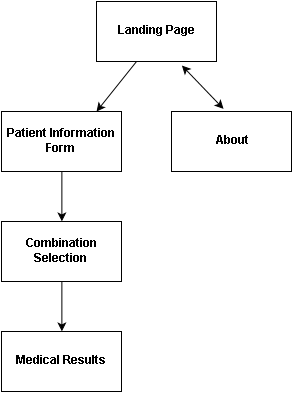
\includegraphics{navflow.png}
  \caption{Application Navigation Flow}
  \label{fig:Application Navigation Flow}
\end{figure}


\end{document}